\begin{itemize}
    \item Directional method for segmented Inverse Beta Decay (IBD) detectors: \\
    \[
    \bar\nu_e + p \to e^+ + n
    \]
    \item Positron (\(e^+\)) gets most of the energy, and annihilation marks prompt vertex
    \item Neutron (\(n\)) gets momentum direction, and capture marks delayed vertex
    \item Lithium 6 dopant localizes \(n\) capture with \({}^3_1\text{H}\) and \({}^4_2\text{He}\) depositing energy within \(\sim10~\mu\)m of capture
    \item direction to source inferred from \(n\) direction with enough events
\end{itemize}

\begin{figure}[ht!]
\centering
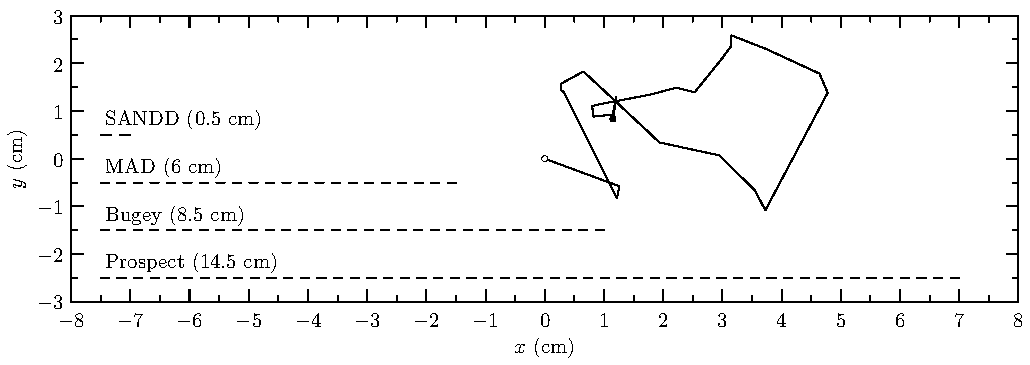
\includegraphics[width=17.405cm,height=7.653cm]{fig/asy_fig_1_paperB.pdf}
    \caption{Diagram showcasing relative scale for characteristic $n~xy$-trajectory projection from IBD vertex to capture location, as well as dimensions of segments in four 2D-segmented detectors: SANDD, MAD, Bugey, and PROSPECT. }
    \label{fig_segmentation_scaling}
\end{figure}